\documentclass[mathserif, table]{beamer}

\usetheme{Boadilla}

\usepackage{subfig}
\usepackage{multirow}
\usepackage{xcolor,colortbl}
\usepackage{listings}
\usepackage{amsmath}

\lstset{language=C,tabsize=4, keepspaces=true,
    xleftmargin=2em,xrightmargin=2em, aboveskip=1em,
    backgroundcolor=\color{lightgray},    % 定义背景颜色
    frame=none,                      % 表示不要边框
    keywordstyle=\color{blue}\bfseries,
    breakindent=22pt,
    numbers=left,stepnumber=1,numberstyle=\tiny,
    basicstyle=\footnotesize,
    showspaces=false,
    flexiblecolumns=true,
    breaklines=true, breakautoindent=true,breakindent=4em,
    escapeinside={/*@}{@*/}
}

% Chinese
\usepackage{ctex}
\setCJKmainfont[BoldFont={SimHei},ItalicFont={KaiTi}]{KaiTi}

% Title
\title{第5章 模拟方法建模}
\author{韩建伟}
\institute{
  信息学院\\
  \texttt{mm@hanjianwei.com}
}
\date{2017/11/10}

\begin{document}

% Title page
\begin{frame}[plain]
  \titlepage{}
\end{frame}

\begin{frame}{为什么要用模拟方法进行建模?}

  \begin{itemize}
  \item 在某些情况下,对对象的行为进行直接观测或重复实验可能是不可行的,如早高峰时电梯系统提供的服务、大城市交通控制系统。
  \item 还有另一些情况,需要对可供选择的模式做试验的系统甚至可能不存在,如一座办公大楼的通讯网络选择、新工厂各台机器的布局、核电站事故防护和疏散方案选择。
  \end{itemize}

  \begin{block}{模拟方法建模}
    当对象的行为不能做分析性的解释,或数据无法直接收集的情况下,建模者可以用某种方式间接地模拟其行为,试验所研究的供选择的各种方案,以估计它们怎样影响对象的行为,然后收集数据来确定哪种方案是最好的。
  \end{block}
\end{frame}

\begin{frame}{蒙特卡罗模拟}
  \begin{block}{Wikipedia.org}
    也称统计模拟方法,是二十世纪四十年代中期由于科学技术的发展和电子计算机的发明,而被提出的一种以概率统计理论为指导的一类非常重要的数值计算方法。是指使用随机数(或更常见的伪随机数)来解决很多计算问题的方法。
  \end{block}

  \begin{figure}
    \centering
    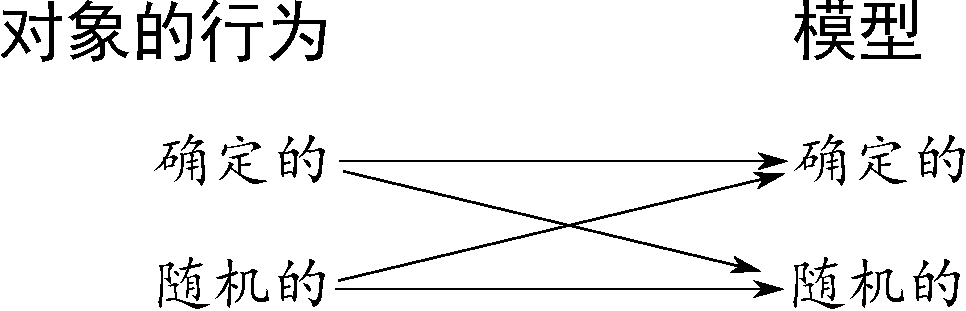
\includegraphics[width=.7\textwidth{}]{action-model.pdf}
  \end{figure}
\end{frame}

\begin{frame}{确定行为的模拟: 曲线下的面积}
  \begin{figure}
    \centering
    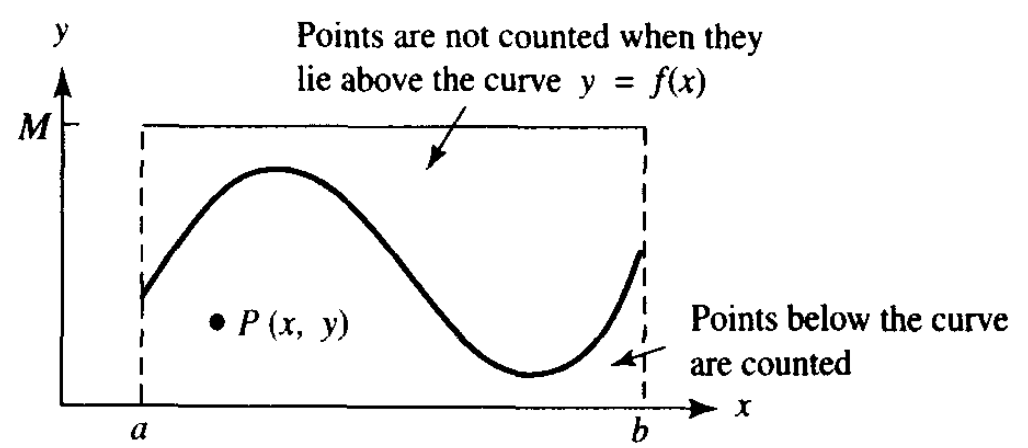
\includegraphics[width=.7\textwidth{}]{curve.png}
  \end{figure}

  \[
  \frac{\text{曲线下的面积}}{\text{矩形面积}} \approx \frac{\text{曲线下的点数}}{\text{随机点的总数}}
  \]
  
\end{frame}

\begin{frame}{计算面积的蒙特卡罗算法}

  \begin{table}
    \centering
    \begin{tabular}{l|l}
      \rowcolor{lightgray}\textbf{输入} & 模拟中产生的随机点总数$n$\\
      \multirow{2}*{\textbf{输出}} & $AREA=$给定区间$a \le x \le b$上曲线$y=f(x)$下的\\
      & 近似面积,其中$0 \le f(x) \le M$.\\
      \rowcolor{lightgray}\textbf{第1步} & 初始化: $COUNTER = 0$\\
      \textbf{第2步} & 对$i = 1, 2, ..., n$, 进行第$3 \sim 5$步\\
      \rowcolor{lightgray}\textbf{\quad{}第3步} & 计算随机坐标$x_i$和$y_i$,满足$a \le x_i \le b$,$0 \le y_i \le M$.\\
      \textbf{\quad{}第4步} & 对随机坐标$x_i$计算$f(x_i)$.\\
      \rowcolor{lightgray}\textbf{\quad{}第5步} & 若$y_i \le f(x_i)$,则COUNTER加1;否则COUNTER不变.\\
      \textbf{第6步} & 计算$AREA=M(b-a)COUNTER/n$\\
      \rowcolor{lightgray}\textbf{第7步} & 输出$(AREA)$\\
      & 停止
    \end{tabular}
  \end{table}
\end{frame}

\begin{frame}{$y=cos(x)$的蒙特卡罗近似}
  \begin{figure}
    \centering
    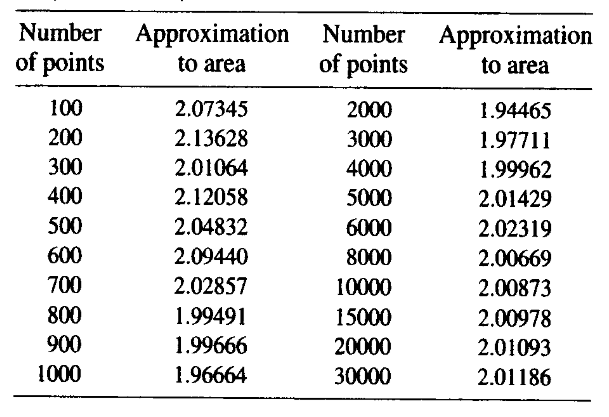
\includegraphics[width=.7\textwidth{}]{cos.png}
    \caption{区间$-\pi/2 \le x \le \pi/2$上曲线$y=cos(x)$下面积的蒙特卡罗近似}
  \end{figure}
\end{frame}

\begin{frame}{曲面下的体积}
  \begin{figure}
    \centering
    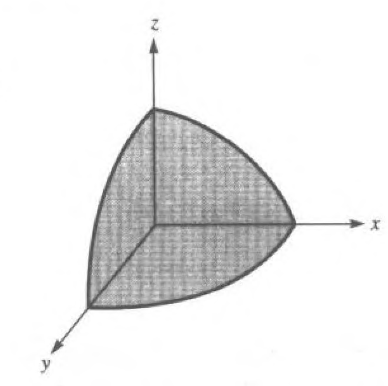
\includegraphics[width=.3\textwidth{}]{sphere.png}
  \end{figure}

  \[
  \frac{\text{曲面下的体积}}{\text{盒子体积}} \approx \frac{\text{第1卦限内曲面下的点数}}{\text{随机点的总数}}
  \]
\end{frame}

\begin{frame}[fragile]{随机数的生成}
  \begin{itemize}
  \item 平方取中方法
  \item 线性同余
  \item C语言中产生0到1之间的随机数
  \end{itemize}

  \begin{lstlisting}[language=C]
    #include <time.h>
    #include <stdio.h>
    #include <stdlib.h>

    int main() {
      float rand_num;
      srand((unsigned)time(NULL));
      rand_num = (float)rand()/RAND_MAX;
      return 0;
    }
  \end{lstlisting}

\end{frame}

\begin{frame}{随机行为的模拟}
  \[
  \text{概率} = \frac{\text{有效事件数}}{\text{事件的总数}}
  \]

  \begin{itemize}
  \item 抛一枚正规的硬币
  \item 掷一个正规的骰子
  \item 掷一个或一对不正规的骰子
  \end{itemize}
  
\end{frame}

\begin{frame}{一枚正规的硬币}
  设$x$是$[0,1]$内的随机数,$f(x)$的定义如下:
  \[
  f(x) =
  \begin{cases}
    \text{正面} & 0 \le x \le 0.5\\
    \text{反面} & 0.5 < x \le 1
  \end{cases}
  \]
\end{frame}

\begin{frame}{抛正规硬币的蒙特卡罗算法}

  \begin{table}
    \centering
    \begin{tabular}{l|l}
      \rowcolor{lightgray}\textbf{输入} & 模拟中产生的随机抛硬币的总次数$n$\\
      \textbf{输出} & 抛硬币时得到正面的概率\\
      \rowcolor{lightgray}\textbf{第1步} & 初始化: $COUNTER = 0$\\
      \textbf{第2步} & 对$i = 1, 2, ..., n$, 进行第$3, 4$步\\
      \rowcolor{lightgray}\textbf{\quad{}第3步} & 得到$[0, 1]$内的随机数.\\
      \multirow{2}*{\textbf{\quad{}第4步}} & 若$0 \le x_i \le 0.5$,则$COUNTER=COUNTER+1$.\\
      & 否则,$COUNTER$不变.\\
      \rowcolor{lightgray}\textbf{第5步} & 计算$P(\text{正面}) = COUNTER/n$\\
      \textbf{第6步} & 输出正面的概率$P(\text{正面})$\\
      \rowcolor{lightgray} & 停止
    \end{tabular}
  \end{table}
\end{frame}

\begin{frame}{结果}
  \begin{figure}
    \centering
    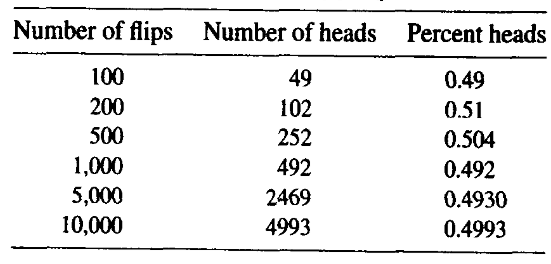
\includegraphics[width=.7\textwidth{}]{coin.png}
  \end{figure}

  扩展:如何用蒙特卡罗方法模拟掷一个正规的骰子?
  
\end{frame}

\begin{frame}{掷一个不正规的骰子}
  \begin{table}
    \centering{}
    \begin{tabular}{|c|c|c|}
      \hline \hline
      $x_i$的值 & 骰子的值 & 出现概率\\
      \hline{}
      $[0,0.1]$ & 1 & 0.1\\
      $(0.1,0.2]$ & 2 & 0.1\\
      $(0.2,0.4]$ & 3 & 0.2\\
      $(0.4,0.7]$ & 4 & 0.3\\
      $(0.7,0.9]$ & 5 & 0.2\\
      $(0.9,1]$ & 6 & 0.1\\
      \hline
    \end{tabular}
  \end{table}
\end{frame}

\begin{frame}{存储模型:汽油与消费需求}
  \begin{block}{问题}
    确定每隔多长时间及把多少汽油运送到各个加油站。每次运送汽油的费用$d$和运送量无关。加油站的需求量可看作常数。如何最小化每天的平均运费,并且每个加油站存储足够的汽油以满足消费需求。
  \end{block}
  \[
  \text{日平均费用} = f(\text{存储费}, \text{运费}, \text{需求率})
  \]
  \begin{description}
  \item[运费] 每次的运费$d$和运送量无关.
  \item[存储费] 单位存储量的费用是常数.
  \item[需求量] 每天的需求量可合理地看作常数.
  \end{description}

\end{frame}

\begin{frame}{常数需求率}
  \begin{figure}
    \centering
    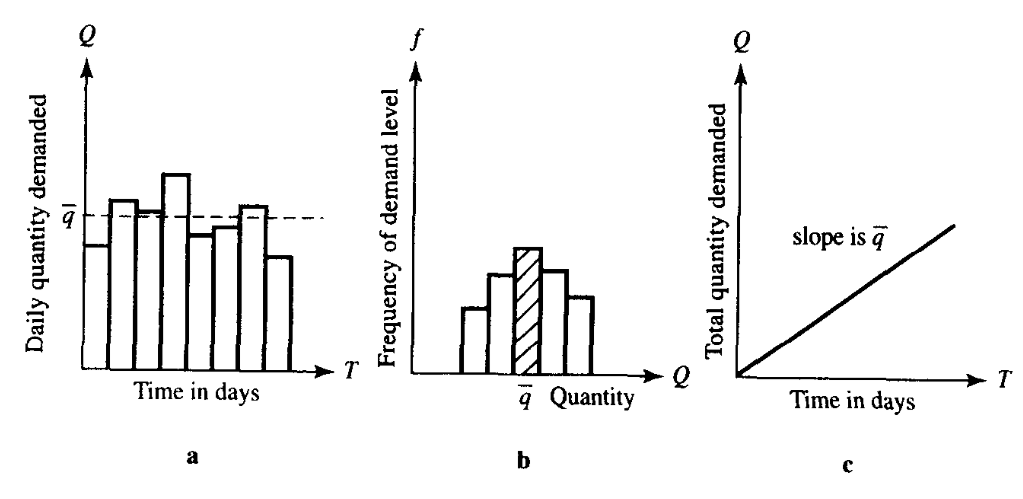
\includegraphics[width=.7\textwidth{}]{gas.png}
  \end{figure}

  在第13章可以得到(符号含义见课本):
  \[
  T^* = \sqrt{\frac{2d}{sr}}
  \]
  \[
  Q^* = rT^*
  \]
\end{frame}

\begin{frame}{需求量的概率统计}
  \begin{figure}
    \begin{tabular}{ccc}
      \hline\hline
      需求量(加仑) & 出现天数 & 出现概率\\
      \hline
      $1000 \sim 1099$ & 10 & 0.01\\
      $1100 \sim 1199$ & 20 & 0.02\\
      $1200 \sim 1299$ & 50 & 0.05\\
      $1300 \sim 1399$ & 120 & 0.12\\
      $1400 \sim 1499$ & 200 & 0.20\\
      $1500 \sim 1599$ & 270 & 0.27\\
      $1600 \sim 1699$ & 180 & 0.18\\
      $1700 \sim 1799$ & 80 & 0.08\\
      $1800 \sim 1899$ & 40 & 0.04\\
      $1900 \sim 1999$ & 30 & 0.03\\
      \hline
      总计 & 1000 & 1.00
    \end{tabular}
    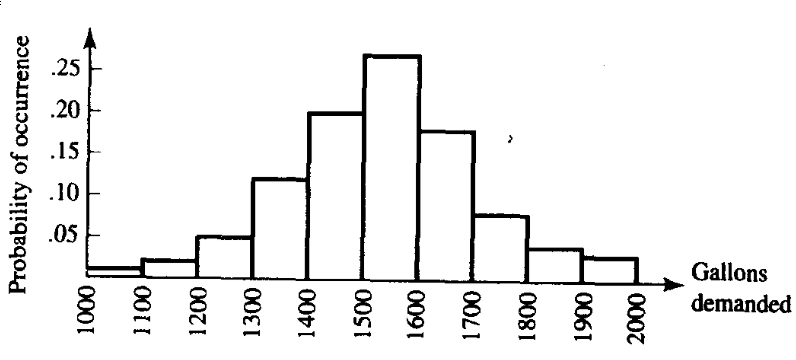
\includegraphics[width=.4\textwidth{}]{gas-freq.png}
  \end{figure}
\end{frame}

\begin{frame}{需求量的累计直方图}
  \begin{figure}
    \setcounter{subfigure}{0}{}
    \subfloat[需求子模型的累计直方图]{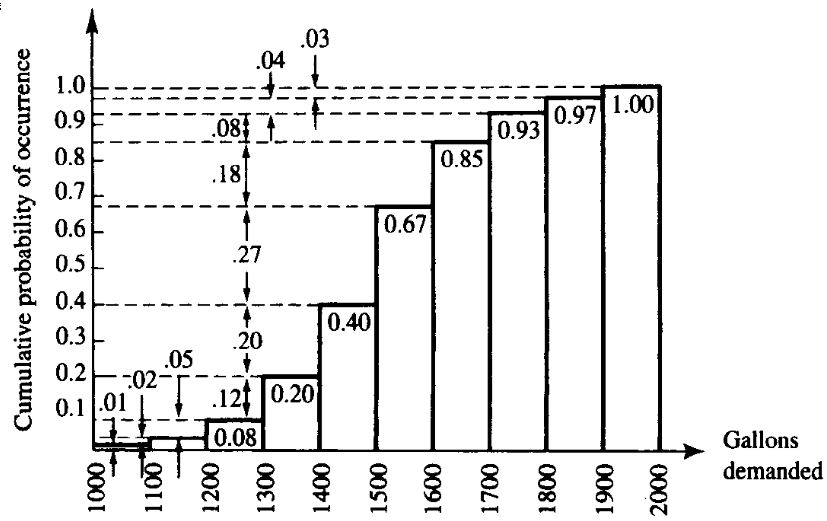
\includegraphics[width=.45\textwidth{}]{gas-distr.png}}
    \subfloat[随机数与需求量的对应关系]{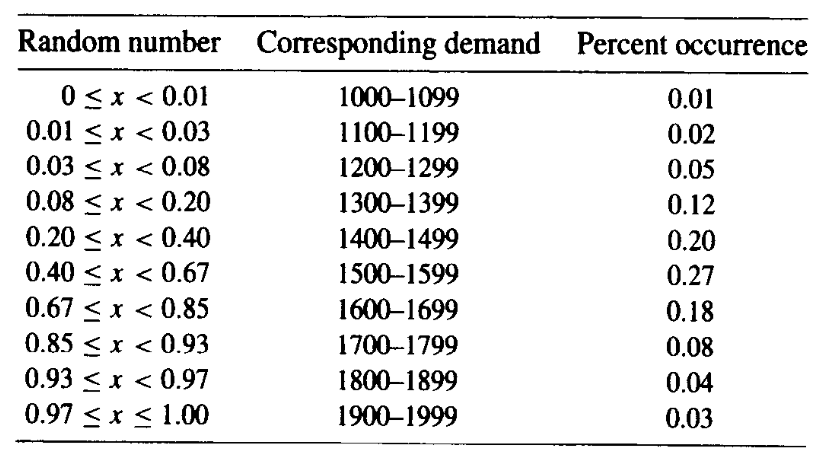
\includegraphics[width=.45\textwidth{}]{gas-occur.png}}
  \end{figure}
\end{frame}

\begin{frame}{需求子模型的蒙特卡罗近似}
  \begin{figure}
    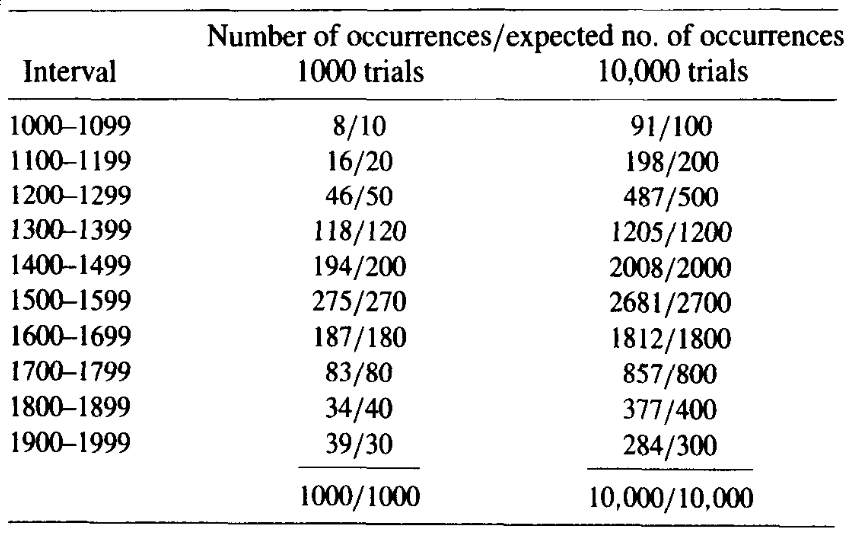
\includegraphics[width=.7\textwidth{}]{gas-mtkl.png}
  \end{figure}  
\end{frame}

\begin{frame}{需求子模型的累计图}
  \begin{figure}
    \setcounter{subfigure}{0}{}
    \subfloat[点表示]{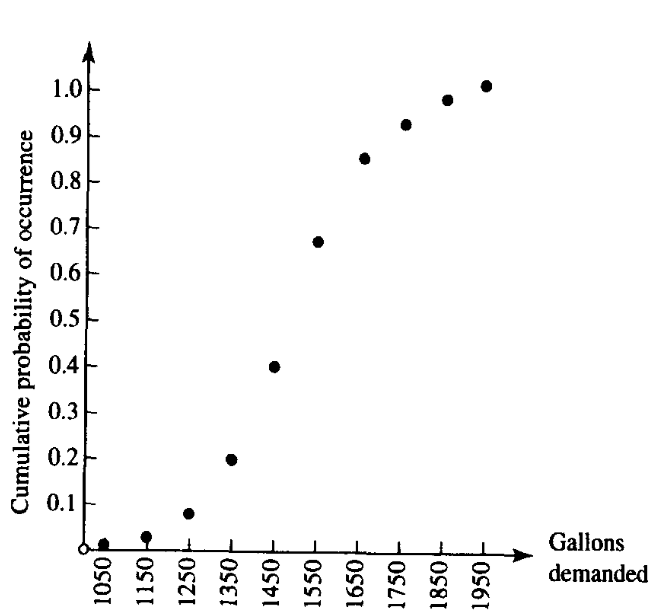
\includegraphics[width=.45\textwidth{}]{gas-point.png}}
    \subfloat[线性样条]{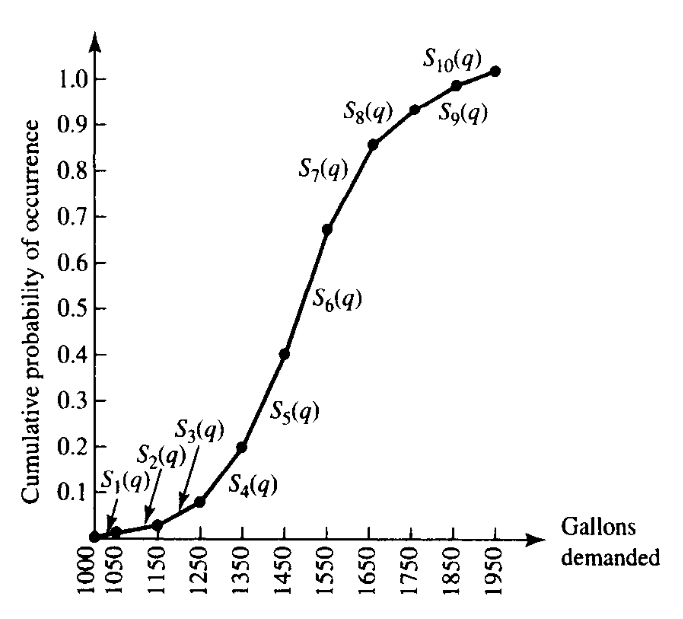
\includegraphics[width=.45\textwidth{}]{gas-spline.png}}
  \end{figure}
\end{frame}

\begin{frame}{蒙特卡罗存储算法术语一览}

  \begin{table}
    \centering
    \begin{tabular}{ll}
      $Q$ & 汽油运量(加仑)\\
      $T$ & 运送的时间间隔(天)\\
      $I$ & 当前的存储量(加仑)\\
      $d$ & 每次运送的费用(元)\\
      $s$ & 每加仑汽油每天的存储费(元)\\
      $C$ & 总费用\\
      $c$ & 每天平均费用\\
      $N$ & 模拟运行的天数\\
      $K$ & 模拟的天数\\
      $x_i$ & $[0,1]$内的随机数\\
      $q_i$ & 日需求量\\
      $Flag$ & 用于中止计算的指标
    \end{tabular}
  \end{table}
  
\end{frame}

\begin{frame}{蒙特卡罗存储算法}

  \begin{table}
    \begin{tabular}{l|l}
      \rowcolor{lightgray}\textbf{输入} & $Q, T, d, s, N$\\
      \textbf{输出} & $c$\\
      \rowcolor{lightgray}& 初始化: \\
      \rowcolor{lightgray}& \quad{}$K = N$\\
      \rowcolor{lightgray}& \quad{}$I = 0$\\
      \rowcolor{lightgray}& \quad{}$C = 0$\\
      \rowcolor{lightgray}\multirow{-5}*{\textbf{第1步}}& \quad{}$Flag = 0$\\
      \multirow{3}*{\textbf{第2步}} & 以一次运送开始下一存储周期:\\
      & \quad{}$I = I + Q$\\
      & \quad{}$C = C + d$\\
      \rowcolor{lightgray}& 确定该存储期的模拟是否中止:\\
      \rowcolor{lightgray}\multirow{-2}*{\textbf{第3步}}& \quad{}若$T \ge K$,置$T = K, Flag = 1$.
    \end{tabular}
  \end{table}
\end{frame}

\begin{frame}{蒙特卡罗存储算法}
  \begin{table}
    \begin{tabular}{l|l}
      \multirow{2}*{\textbf{第4步}} & 模拟这个存储期(或剩余部分)的每一天\\
      & \quad{}对于$i = 1, 2, ..., T$,执行第$5 \sim 9$步.\\
      \rowcolor{lightgray}\textbf{\quad{}第5步} & 生成随机数$x_i$\\
      \textbf{\quad{}第6步} & 利用需求子模型计算$q_i$\\
      \rowcolor{lightgray}\textbf{\quad{}第7步} & 修正当前的存储量$I=I-q_i$\\
      \multirow{3}*{\textbf{\quad{}第8步}} & 若存储量用完,即$I \le 0$,置$I = 0$,转第9步;\\
      & 否则,计算日存储费和总费用:\\
      & \quad{}$C = C + I*s$\\
      \rowcolor{lightgray}& 减少模拟中剩下的天数\\
      \rowcolor{lightgray}\multirow{-2}*{\textbf{\quad{}第9步}} & \quad{}$K = K - 1$
    \end{tabular}
  \end{table}
  
\end{frame}

\begin{frame}{蒙特卡罗存储算法}
  \begin{table}
    \begin{tabular}{l|l}
      \textbf{第10步} & 若$Flag = 0$,转第2步;否则,转第11步\\
      \rowcolor{lightgray}\textbf{第11步} & 计算每天平均费用$c = C/N$\\
      \textbf{第12步} & 输出$c$\\
       \rowcolor{lightgray}& 停止
    \end{tabular}
  \end{table}
  
\end{frame}

\begin{frame}{排队模型}
  \begin{block}{港口系统} 一个只能同时为1只船卸货的港口,相邻两艘船到达的时间间隔在15分钟到145分钟之间变化,每艘船的卸货时间在45分钟到90分钟之间变化,需要回答以下问题:
  \end{block}

  \begin{itemize}
  \item 每艘船只在港口的平均时间和最长时间是多少?
  \item 平均等待时间和最长等待时间是多少?
  \item 卸货设备空闲的时间百分比是多少?
  \item 船只排队最长的长度是多少?
  \end{itemize}

\end{frame}

\begin{frame}{5艘船只的例子}
  \begin{figure}
    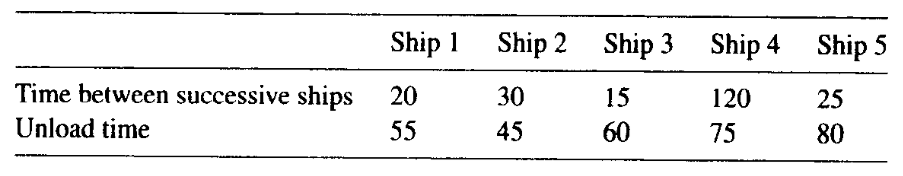
\includegraphics[width=.7\textwidth{}]{ships.png}\\
    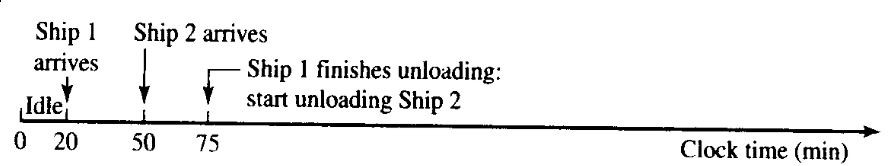
\includegraphics[width=.5\textwidth{}]{ship-t1.png}
    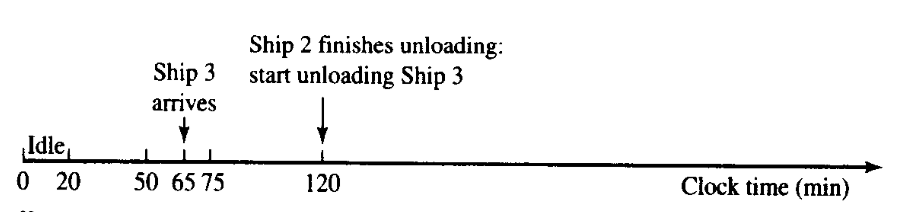
\includegraphics[width=.5\textwidth{}]{ship-t2.png}\\
    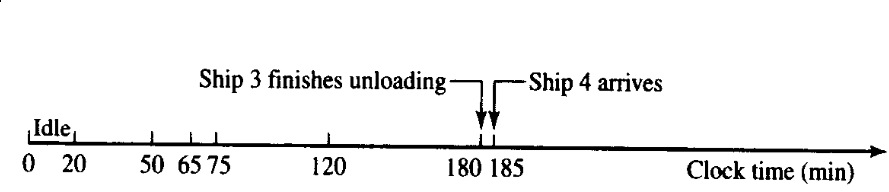
\includegraphics[width=.5\textwidth{}]{ship-t3.png}
    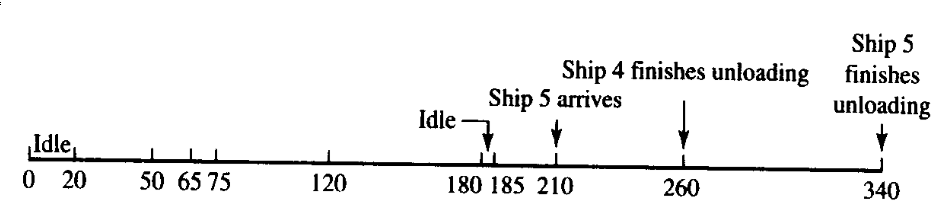
\includegraphics[width=.5\textwidth{}]{ship-t4.png}
  \end{figure}  
  
\end{frame}

\begin{frame}{模拟概要}
  \begin{figure}
    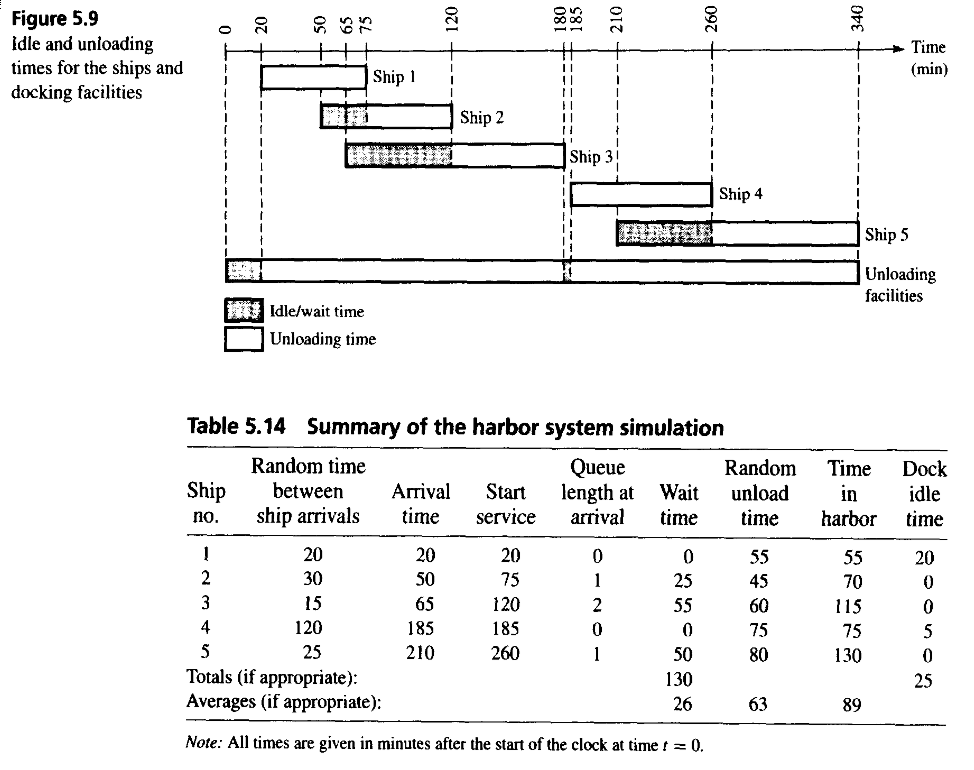
\includegraphics[height=.85\textheight{}]{ship-summary.png}
  \end{figure}  

\end{frame}

\begin{frame}{港口系统算法术语一览}

  \begin{table}
    \centering
    \begin{tabular}{ll}
      $between_i$ & 船$i$与$i-1$的到达时间间隔(15-145之间的随机整数)\\
      $arrive_i$  & 从时钟t=0分开始计时,船$i$到达港口的时间\\
      $unload_i$  &  船$i$在港口卸货所需的时间(45和90之间的随机整数)\\
      $start_i$    &  船$i$开始卸货的时间\\
      $idle_i$     &  恰在船$i$开始卸货之前码头设备空闲的时间\\
      $wait_i$     &  船$i$到达后开始卸货前在码头的等待时间\\
      $finish_i$   &   船$i$卸货完毕的时间\\
      $harbor_i$   &  船$i$呆在港口的总的时间\\
    \end{tabular}
  \end{table}
\end{frame}

\begin{frame}{港口系统算法术语一览}

  \begin{table}
    \centering
    \begin{tabular}{ll}
      $HARTIME$ & 每艘船呆在港口的平均时间\\
      $MAXHAR$ & 一艘船呆在港口的最长时间\\
      $WAITIME$ &  每艘船卸货之前的平均等待时间\\
      $MAXWAIT$ & 一艘船的最长等待时间\\
      $IDLETIME$ &  卸货设备空闲时间占总模拟时间的百分比
    \end{tabular}
  \end{table}
\end{frame}
    
\begin{frame}{港口系统模拟算法}
  \begin{table}
    \begin{tabular}{l|l}
      \textbf{输入} &    模拟中的船只总数$n$\\
      \rowcolor{lightgray}\textbf{输出} &    $HARTIME$, $MAXHAR$,$WAITIME$, $MAXWAIT$,$IDLETIME$\\
      \textbf{第1步} &  随机生成$between_1$和$unload_1$,令$arrive_1=between_1$\\
      \rowcolor{lightgray}&  全部输出初始化:\\
      \rowcolor{lightgray}& \quad{}$HARTIME=unload_1,  MAXHAR=unload_1$\\
      \rowcolor{lightgray}\multirow{-3}*{\textbf{第2步}}& \quad{}$WAITME=0, MAXWAIT=0, IDLETIME=arrive_1$\\
      \multirow{2}*{\textbf{第3步}} &  计算船1卸货完毕的时间:\\
      & \quad{}$finish_1=arrive_1+unload_1$\\
      \rowcolor{lightgray}\textbf{第4步} &   对于$i=2,3, …, n$, 执行第5-16步\\
      \textbf{\quad{}第5步} &  分别在各自的区间上生成一对随机整数$between_i$和$unload_i$
    \end{tabular}
  \end{table}


\end{frame}

\begin{frame}{港口系统模拟算法}
  \begin{table}
    \begin{tabular}{l|l}
      \rowcolor{lightgray} & 假定时钟从$t=0$分钟开始计时,计算船$i$的到达时间\\
      \rowcolor{lightgray}\multirow{-2}*{\textbf{\quad{}第6步}} & \quad{}$arrive_i=arrive_{i-1}+between_i$\\
      \multirow{2}*{\textbf{\quad{}第7步}} & 计算船$i$到达与船$i-1$卸货完毕的时间之差:\\
      & \quad{}$timediff=arrive_i-finish_{i-1}$\\
      \rowcolor{lightgray} &   若timediff非负,则卸货设备空闲:\\
      \rowcolor{lightgray} & \quad{}$idlei=timediff$且$waiti=0$\\
      \rowcolor{lightgray} &若timediff为负,则船$i$在卸货前必须等待:\\
      \rowcolor{lightgray} \multirow{-4}*{\textbf{\quad{}第8步}} & \quad{}$waiti= -timediff$且$idlei = 0$\\
      \multirow{2}*{\textbf{\quad{}第9步}} &   计算船$i$开始卸货的时间\\
      & \quad{}$starti=arrive_i+waiti$
    \end{tabular}
  \end{table}
\end{frame}

\begin{frame}{港口系统模拟算法}
  \begin{table}
    \begin{tabular}{l|l}
      \rowcolor{lightgray} &  计算船$i$卸货完毕的时间\\
      \rowcolor{lightgray} \multirow{-2}*{\textbf{\quad{}第10步}} & \quad{} $finish_i=start_i +unload_i$\\
      \multirow{2}*{\textbf{\quad{}第11步}} &   计算船只呆在港口的时间\\
      & \quad{}$harbor_i=wait_i+unload_i$\\
      \rowcolor{lightgray}\textbf{\quad{}第12步} &   将$harbor_i$加入总的港口时间$HARTIME$,平均时用到\\
      \multirow{2}*\textbf{\quad{}第13步} &   若$harbor_i>MAXHAR$,则令$MAXHAR=harbor_i$;\\
      & 否则$MAXHAR$不变\\
      \rowcolor{lightgray}\textbf{\quad{}第14步} &   将$wait_i$加入总的等待时间$WAITIME$,平均时用到\\
      \textbf{\quad{}第15步} &  将$idle_i$加入总的空闲时间$IDLETIME$\\
      \rowcolor{lightgray} &   若$wait_i>MAXWAIT$,则令$MAXWAIT=wait_i$;\\
      \rowcolor{lightgray}\multirow{-2}*{\textbf{\quad{}第16步}} & 否则$MAXWAIT$不变\\
    \end{tabular}
  \end{table}
\end{frame}

\begin{frame}{港口系统模拟算法}
  \begin{table}
    \begin{tabular}{l|l}
      \multirow{2}*{\textbf{第17步}} &   令$HARTIME=HATIME/n, WAITIME=WAITIME/n$,\\
      & 且$IDLETIME=IDLETIME/finish_n$\\
      \rowcolor{lightgray} & 输出$(HARTIE,MAXHAR,WAITIME,$\\
      \rowcolor{lightgray}\multirow{-2}*{\textbf{第18步}} & \quad{}\quad{}\quad{}$MAXWAIT,IDLETIME)$\\
      & 停止 
    \end{tabular}
  \end{table}
\end{frame}

\begin{frame}{模拟结果}

  \begin{figure}
    \centering
    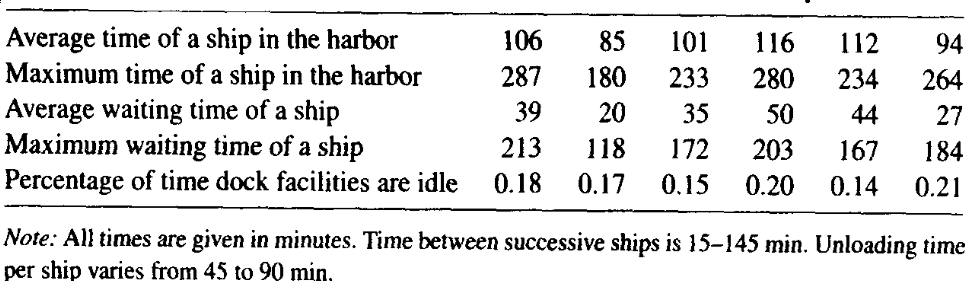
\includegraphics[height=.25\textheight{}]{harbor-sim.png}\\
    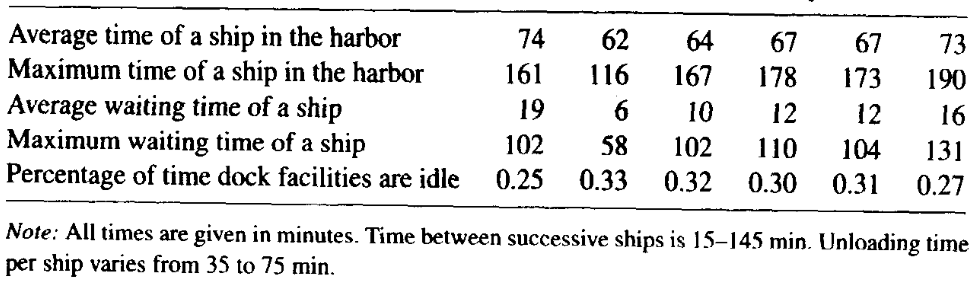
\includegraphics[height=.25\textheight{}]{harbor-sim2.png}\\
    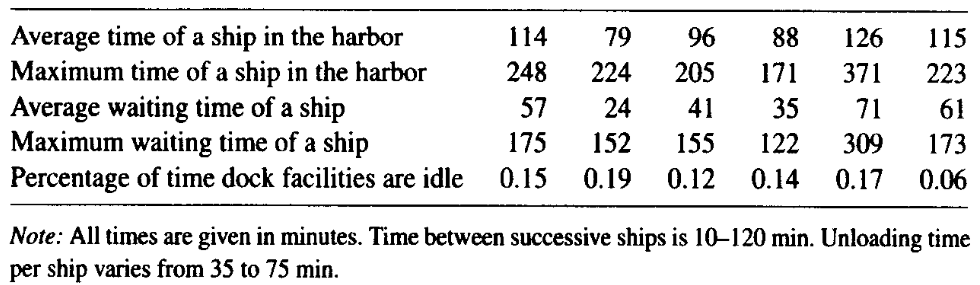
\includegraphics[height=.25\textheight{}]{harbor-sim3.png}
  \end{figure}
  
\end{frame}

\begin{frame}{搜集港口数据}
  \begin{figure}
    \centering
    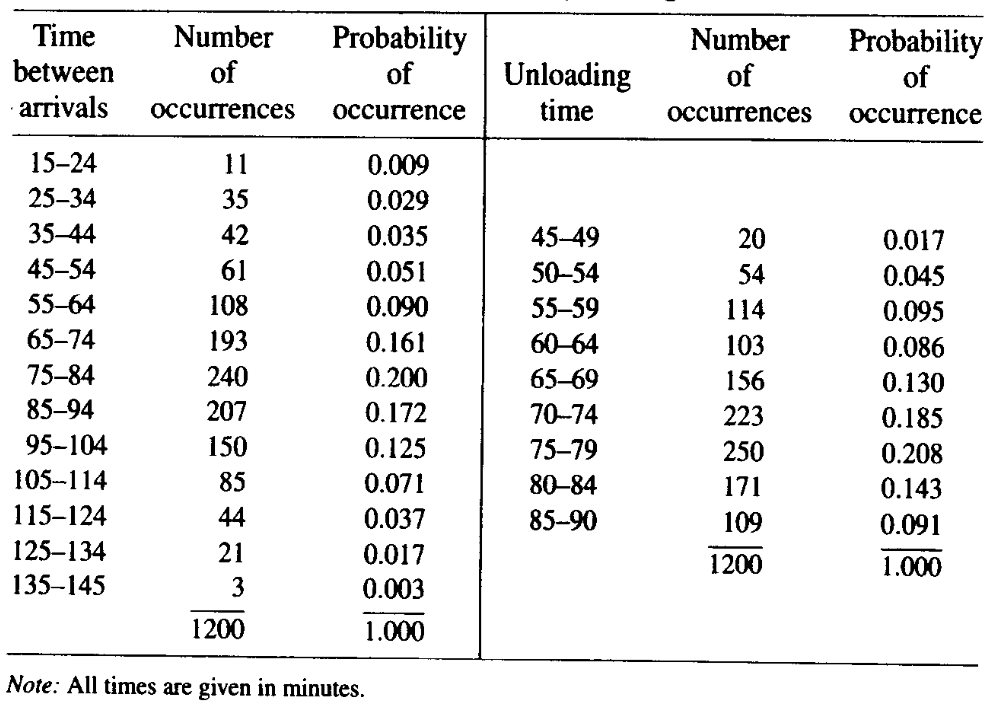
\includegraphics[width=.8\textwidth{}]{harbor-real.png}
  \end{figure}
  
\end{frame}

\begin{frame}{累计直方图}

  \begin{figure}
    \centering
    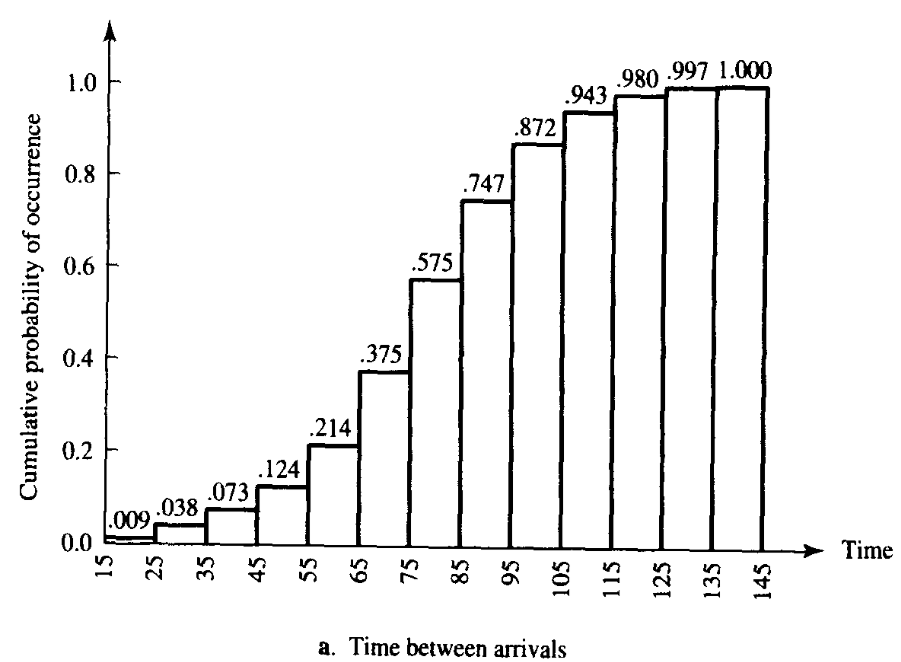
\includegraphics[height=.5\textheight{}]{harbor-arrive.png}
    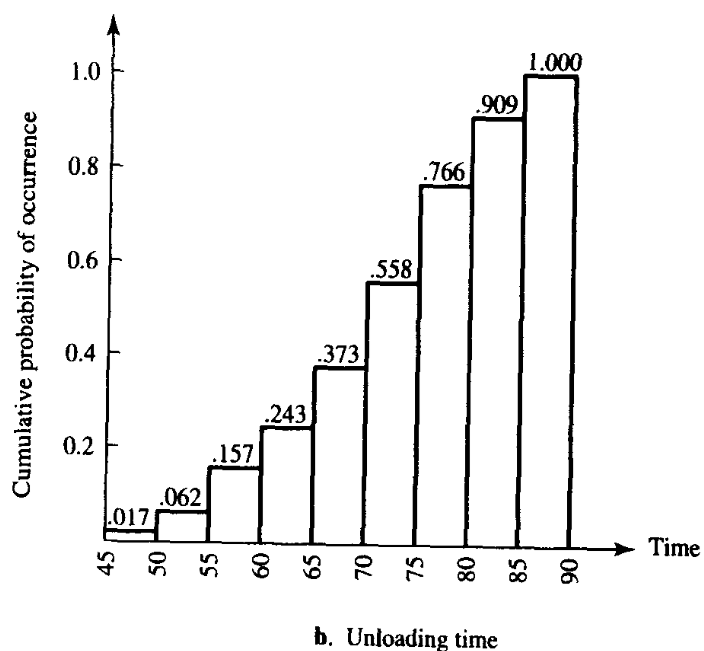
\includegraphics[height=.5\textheight{}]{harbor-unload.png}
  \end{figure}
  
\end{frame}

\begin{frame}{基于直方图的模拟结果}
  \begin{figure}
    \centering
    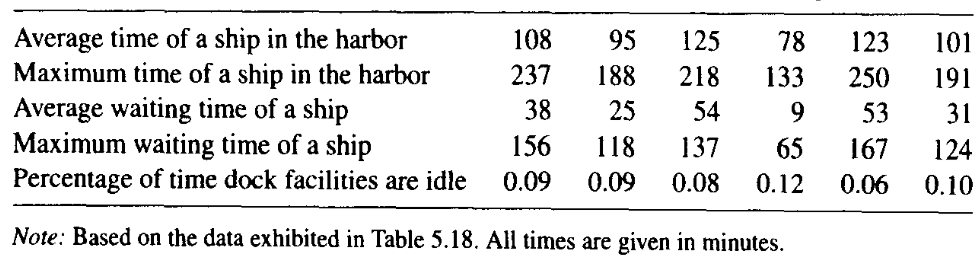
\includegraphics[width=.8\textwidth{}]{harbor-sim-real.png}
  \end{figure}
  
\end{frame}

\begin{frame}{扩展}

早高峰时间的电梯调度算法.
  
\end{frame}

\end{document}

%%% Local Variables: 
%%% TeX-master: t
%%% TeX-engine: xetex
%%% End: 
